\documentclass[12pt, twoside]{report}
	\usepackage[right=1.2in, left = 1.1in, top=1in, bottom=1in]{geometry}
	\usepackage[hidelinks, linktoc=all, pagebackref, russian]{hyperref}
	\usepackage{indentfirst}
    \usepackage[russian]{babel}
    \usepackage{subcaption}
    \captionsetup[subfigure]{justification=centering}
   	\usepackage[superscript,biblabel]{cite}
    \usepackage[font=small,labelfont=bf]{caption}
    \usepackage{abstract}
    \usepackage{mathtools}
    \usepackage{fancyhdr}
    \usepackage{bbm}
    \usepackage{cleveref}
    \setlength{\parskip}{0.1cm}   
	\setlength{\parindent}{0.7cm}
    \usepackage{graphicx} % Used to insert images
    \usepackage{adjustbox} % Used to constrain images to a maximum size 
   	\usepackage{color} % Allow colors to be defined
    \usepackage{enumerate} % Needed for markdown enumerations to work
    \usepackage{geometry} % Used to adjust the document margins
    \usepackage{amsmath} % Equations
    \usepackage{amssymb} % Equations
    \usepackage[mathletters]{ucs} % Extended unicode (utf-8) support
    \usepackage[utf8x]{inputenc} % Allow utf-8 characters in the tex document
    \usepackage{fancyvrb} % verbatim replacement that allows latex
    \usepackage{grffile} % extends the file name processing of package graphics 
                         % to support a larger range 
    % The hyperref package gives us a pdf with properly built
    % internal navigation ('pdf bookmarks' for the table of contents,
    % internal cross-reference links, web links for URLs, etc.)
    \usepackage{longtable} % longtable support required by pandoc >1.10


 	
\addto\extrasrussian{%
  \renewcommand{\figureautorefname}{Рис.}%
}
\newcommand{\Tr}[1]{\text{Tr}\left[#1\right]}
\newcommand{\pTr}[2]{\text{Tr}_{#1}\left[#2\right]}

\DeclarePairedDelimiter\bra{\langle}{\rvert}
\DeclarePairedDelimiter\ket{\lvert}{\rangle}
\DeclarePairedDelimiterX\braket[2]{\langle}{\rangle}{#1 \delimsize\vert #2}
\newcommand{\rbrkt}[1]{\left( #1 \right)}
\newcommand{\sbrkt}[1]{\left[ #1 \right]}
\renewcommand*{\backreftwosep}{ и~}
\renewcommand*{\backreflastsep}{ и~}
\renewcommand*{\backref}[1]{}
\renewcommand*{\backrefalt}[4]{%
\ifcase #1 %
\relax%
\or
(ссылка на стр. [#2])%
\else
(ссылки на стр. [#2])%
\fi
}

\numberwithin{equation}{section}
\renewcommand*\thesection{\arabic{section}}
\lhead[\rm\thepage]{\fancyplain{}{\nouppercase{\sl{\rightmark}}}}
\rhead[\fancyplain{}{\nouppercase{\sl{\leftmark}}}]{\rm\thepage}
\chead{}\lfoot{}\rfoot{}\cfoot{}
\pagestyle{fancy}

	\author{Федоров Глеб, 125}
 	\title{Диплом}

\begin{document}
\maketitle
\tableofcontents
\newpage
\chapter{Введение}
Квантовый компьютер -- это устройство, хранящее и обрабатывающее информацию внутри группы квантовых систем, причем обработка информации происходит в результате когерентных взаимодействий систем внутри группы \cite{Lloyd1993}. Каждая квантовая система, как правило, является двухуровневой и носит название ``квантовый бит'' или ``кубит'' (англ. ``qubit'' -- quantum bit). Для осуществления квантового расчета необходимо связать кубиты друг с другом, иметь возможность управлять состоянием кубитов и считывать его, сохраняя чистоту соответствующей матрицы плотности, а также обеспечить изоляцию кубитов от влияния окружающей среды. Следовательно, в качестве кубитов могут быть использованы любые достаточно изолированные двухуровневые системы, поддающиеся контролю и способные взаимодействовать друг с другом \cite{DiVincenzo1995, DiVincenzo2000, Spiller1996}. В качестве примера можно привести фотоны \cite{Milburn2009}, ионы в ионных ловушках \cite{Cirac1995}, ядерные спины \cite{Kane1998}, атомы в электромагнитных резонаторах\cite{Rempe2008},  электрические системы\cite{Devoret2005} и т.п.

Последние являются одними их самых заманчивых кандидатов на эту роль, но при условии, что их поведение будет именно квантовым, а не классическим\cite{Devoret1995}. К счастью, явление сверхпроводимости и эффект Джозефсона позволяют наблюдать квантовые эффекты в контурах даже мезоскопического масштаба и создавать на их основе так называемые \textit{сверхпроводящие (джозефсоновские) кубиты}\cite{Clarke2008}. В данной работе проводится исследование одного из них -- потокового сверхпроводящего кубита (он был впервые предложен в статье\cite{Orlando1999} и назван Flux-кубитом).

Джозефсоновские кубиты имеют два значительных недостатка и одно значительное преимущество в сравнении с микроскопическими кубитами. Первый недостаток заключается в значительном взаимодействии с окружающей средой - в силу больших размеров, джозефсоновские кубиты сильнее связываются со средой, что требует дополнительных изысканий в области их изоляции; второй недостаток заключается в том, что в то время как микроскопические кубиты, например, атомы, идентичны друг другу, сверхпроводящие кубиты могут иметь отличия из-за неточностей производства. Для борьбы с этим требуется либо создавать заведомо нечувствительные к дефектам схемы, либо проводить калибровку, в процессе которой параметры цепей измеряются, а затем компенсируются в эксперименте.

Преимущество джозефсоновских кубитов в их гибкости: они могут быть произвольным образом расположены относительно друг друга, а их параметры легко и непрерывно изменяемы в широких пределах. Эта гибкость вместе с некоторыми фундаментальными эффектами\cite{Koch2007} может быть использована для борьбы с первым недостатком, а также предоставляет много вариантов для подстройки параметров, что в значительной степени нивелирует второй недостаток. Далее, накопленный опыт человечества в области изготовления интегральных схем позволит упростить переход к производству реальных квантовых вычислительных устройств, что является еще одним преимуществом в сравнении с другими типами кубитов. Таким образом, скорее всего именно джозефсоновские кубиты и будут применены в первом квантовом компьютере, и именно их следует изучать.

Важно отметить, что сверхпроводящие кубиты могут применяться не только для непосредственного использования в квантовом компьютере, так как по сути являются рукотворными атомами с широко изменяемыми характеристиками, как внутренними, так и касающимися связи с окружением. Они могут быть пригодны для создания метаматериалов \cite{Macha2014}, проведения высокоточных измерений полей\cite{Clarke2006}, использоваться в качестве активной среды\cite{Astafiev2010}, применяться в квантовой криптографии и телепортации \cite{Xia2014} и т.п. 
\newpage
\chapter{Теоретические сведения}
Данный раздел содержит теоретическое описание явлений, наблюдаемых в экспериментальной части работы. Далее будут кратко рассмотрена теория сверхпроводимости, эффект Джозефсона, затем произведено рассмотрение теории изолированного Flux-кубита, теории его взаимодействия с окружающей средой и, наконец, вопросы измерения и контроля. 
\section{Явление сверхпроводимости}
Сверхпроводимость -- это сложное коллективное явление, свойство некоторых материалов обладать строго нулевым электрическим сопротивлением при достижении ими температуры ниже определенного значения. В настоящий момент самой известной точной теорией сверхпроводимости является теория БКШ\cite{Schrieffer1999}, согласно которой электроны в сверхпроводнике при переходе через критическую температуру объединяются в так называемые куперовские пары и претерпевают бозе-конденсацию. Спаривание электронов происходит в результате обмена фононами, приводящего к эффективному притяжению между ними и образованию связанного состояния на уровне Ферми, отделенного от уровней квазичастичных возбуждений энергетической щелью. Полное описание данного эффекта в рамках микроскопической теории невозможно в данной работе, поэтому мы будем далее пользоваться феноменологической теорией Гинзбурга-Ландау \cite{GL1950}, которая выводится из модели БКШ\cite{Gorkov1959}, но является более удобной в практическом применении. Сверхпроводящее состояние в рамках этой теории может быть описано параметром порядка или, иначе, модулем так называемой "макроскопической волновой функции куперовских пар":
\begin{equation}
\Psi(\mathbf{r}) = \sqrt{\frac{n_s}{2}}e^{i\theta(\mathbf{r})},
\label{eq:glwf} 
\end{equation}
где $n_s$ -- концентрация сверхпроводящих электронов в сверхпроводнике. Важно подчеркнуть, что она не является настоящей волновой функцией, но тем не менее позволяет получить практически важные результаты. Мы далее считаем, что в изолированном невозмущенном полями сверхпроводнике и модуль, и фаза волновой функции (\ref{eq:glwf}) постоянны.

Из минимизации функционала Гинзбурга-Ландау и одного из уравнений Максвелла можно получить следующее уравнение для сверхпроводящего тока куперовских пар в зависимости от приложенного поля, являющееся обобщением уравнения Лондонов:
\begin{equation}
\mathbf{j}_s = -\frac{i\hbar e}{2m_e}(\Psi^*\nabla\Psi - \Psi\nabla\Psi^*) - \frac{2e^2}{m_e}\mathbf{A}|\Psi|^2.
\label{eq:lond}
\end{equation}
Подставляя сюда $\Psi(\mathbf{r})$ из определения (\ref{eq:glwf}), получим:
\begin{equation}
\mathbf{j}_s = \frac{1}{\Lambda}\left(\frac{\Phi_0}{2\pi}\nabla\theta(\mathbf{r})-\mathbf{A}\right),
\label{eq:lond2}
\end{equation}
где $\displaystyle \Lambda = \frac{m_e}{n_s e^2},\ \Phi_0 = \frac{h}{2e}$. Вторая константа, как будет показано далее, является \textit{квантом магнитного потока}, и имеет важное значение в данной работе.
\section{Эффект Джозефсона}
\subsection{Уравнения Джозефсона}
Эффект Джозефсона\cite{Josephson1964} -- это эффект установления одной макроскопической фазы в двух сверхпроводниках, соединенных через так называемую ``слабую связь''. Слабые связи многообразны: это могут быть тонкие слои диэлектрика, сужения, точечные контакты, прослойки из металла в нормальном состоянии или из ферромагнетика. В случае, если фазы не равны, то через слабую связь будет течь бездиссипативный ток, и будет выполнено некоторое \textit{фазо-токовое соотношение} между током и скачком фазы на переходе. Часто, хотя и не всегда\cite{Golubov2004}, оно оказывается синусоидальным:
\begin{equation}
I_s = I_c \sin(\theta_2 - \theta_1) = I_c \sin\varphi.
\label{eq:CPR}
\end{equation}
Из этой формулы видно, что сверхпроводящий ток $I_s$ не может превысить некоторого значения $I_c$. Это так называемый \textit{критический ток} джозефсоновского перехода, при превышении которого бездиссипативность нарушается, и на переходе устанавливается напряжение V. В этом случае выполнено второе уравнение Джозефсона:
\begin{equation}
\hbar \frac{\partial \varphi}{\partial t} = 2eV,
\label{eq:2JE}
\end{equation}
и наблюдаются осцилляции разности фаз между сверхпроводниками. Величина критического тока рассчитывается из микроскопической теории, например, для перехода SIS верна формула Амбегаокара-Баратова:
\begin{equation}
I_c = \frac{\pi\Delta(T)}{2eR_n}\th\left(\frac{\Delta(T)}{2k_bT}\right),
\label{eq:Ic}
\end{equation}
где через $T$ обозначена температура, а через $R_n$ сопротивление контакта в отсутствие сверхпроводимости, $R_n = \rho\frac{d}{S}$, где $\rho$ -- удельное сопротивление I-слоя, а $d$ и $S$ -- его толщина и площадь.
\subsection{RCSJ-модель}
Для упрощения описания динамики джозефсоновского контакта применяется модель RCSJ (Resistively and Capacitively Shunted Junction), работающая для маленьких переходов со слоем изолятора, когда изменения фазы на размере контакта пренебрежимо малы и присутствует ненулевая геометрическая емкость. 
\begin{figure}[h]
\centering
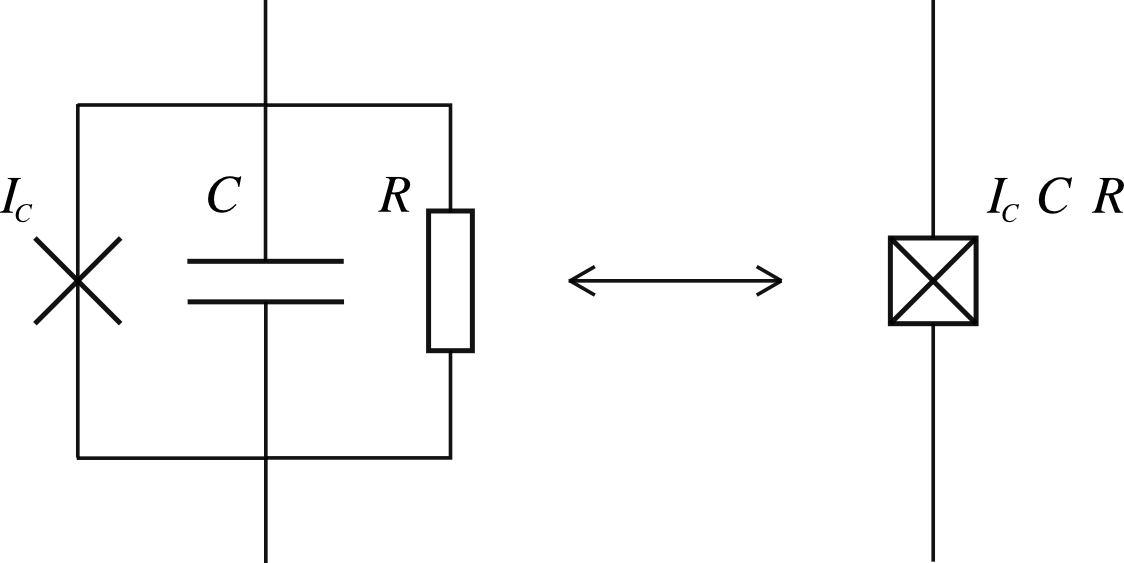
\includegraphics[width=0.65\textwidth]{Pictures/RCSJ.png}
\caption{Схема RCSJ в виде параллельного соединения идеального джозефсоновского перехода с конденсатором и резистором.}
\label{fig:RSCJ}
\end{figure}

Принципиальная схема изображена на \autoref{fig:RSCJ}. В случае, когда ток через систему не превышает критического $I_c$, резистор на схеме может быть опущен. В силу параллельности соединения выполнено также соотношение $\displaystyle \frac{\hbar}{2e}\frac{\partial\varphi}{\partial t} = U_C$ между напряжениями на переходе и на конденсаторе, которое устанавливает аналогию между неидеальным переходом и колебательным контуром с нелинейной индуктивностью.

В рамках RCSJ-модели энергия перехода состоит из энергии, запасенной в нелинейной индуктивности идеального перехода, и энергии конденсатора:
\begin{gather}
E = E_{ind}+E_{cap}  \label{eq:JJenrj1}\\
E_{ind} = \int I_JV_J\, dt = I_c \frac{\hbar}{2e}\int_0^T \sin(\phi(t))\frac{d\phi(t)}{dt}dt \notag\\
= E_J \int_0^\varphi \sin\phi\, d\phi = E_J [1-\cos\varphi] \\
E_{cap} = \frac{1}{2}C U_C^2 = \frac{1}{2} C \left(\frac{\Phi_0}{2\pi}\right)^2 \dot \varphi^2 = 
\frac{\hbar^2}{4E_C} \dot \varphi^2,\ E_C = \frac{(2e)^2}{2C}.
\label{eq:JJenrj2}
\end{gather}
\subsection{Фазо-потоковое соотношение}
Рассмотрим замкнутый сверхпроводящее кольцо конечной толщины, быть может, прерванный конечным числом джозефсоновских переходов $\{J_1..J_n\}$. Рассмотрим применительно к данному случаю уравнение (\ref{eq:lond2}). Проведем контур $C$ внутри кольца так, чтобы он нигде не приближался к стенкам на расстояние, меньшее глубины проникновения магнитного поля (\autoref{fig:ring}). Тогда сверхток на всей его длине будет равен нулю, и, проинтегрировав по нему (\ref{eq:lond2}), мы получим следующее равенство:
\begin{equation}
\oint\displaylimits_C \mathbf{A}d\mathbf{l} = \frac{\Phi_0}{2\pi}\oint\displaylimits_C \nabla \theta d \mathbf{l} \notag.
\end{equation}
Руководствуясь \autoref{fig:ring}, соображениями однозначности волновой функции (\ref{eq:glwf}) при обходе вокруг контура и теоремой Стокса для $\operatorname{rot} \mathbf{A}$, можем написать:
\begin{gather}
\Phi = \frac{\Phi_0}{2\pi}\left(\sum_i \varphi_n + 2\pi k\right) \notag \\
\sum_i \varphi_n = 2\pi\left(\frac{\Phi}{\Phi_0} - k\right),\ k\in \mathcal{Z}.
\label{eq:phsflx}
\end{gather}

\begin{figure}[h]
\centering
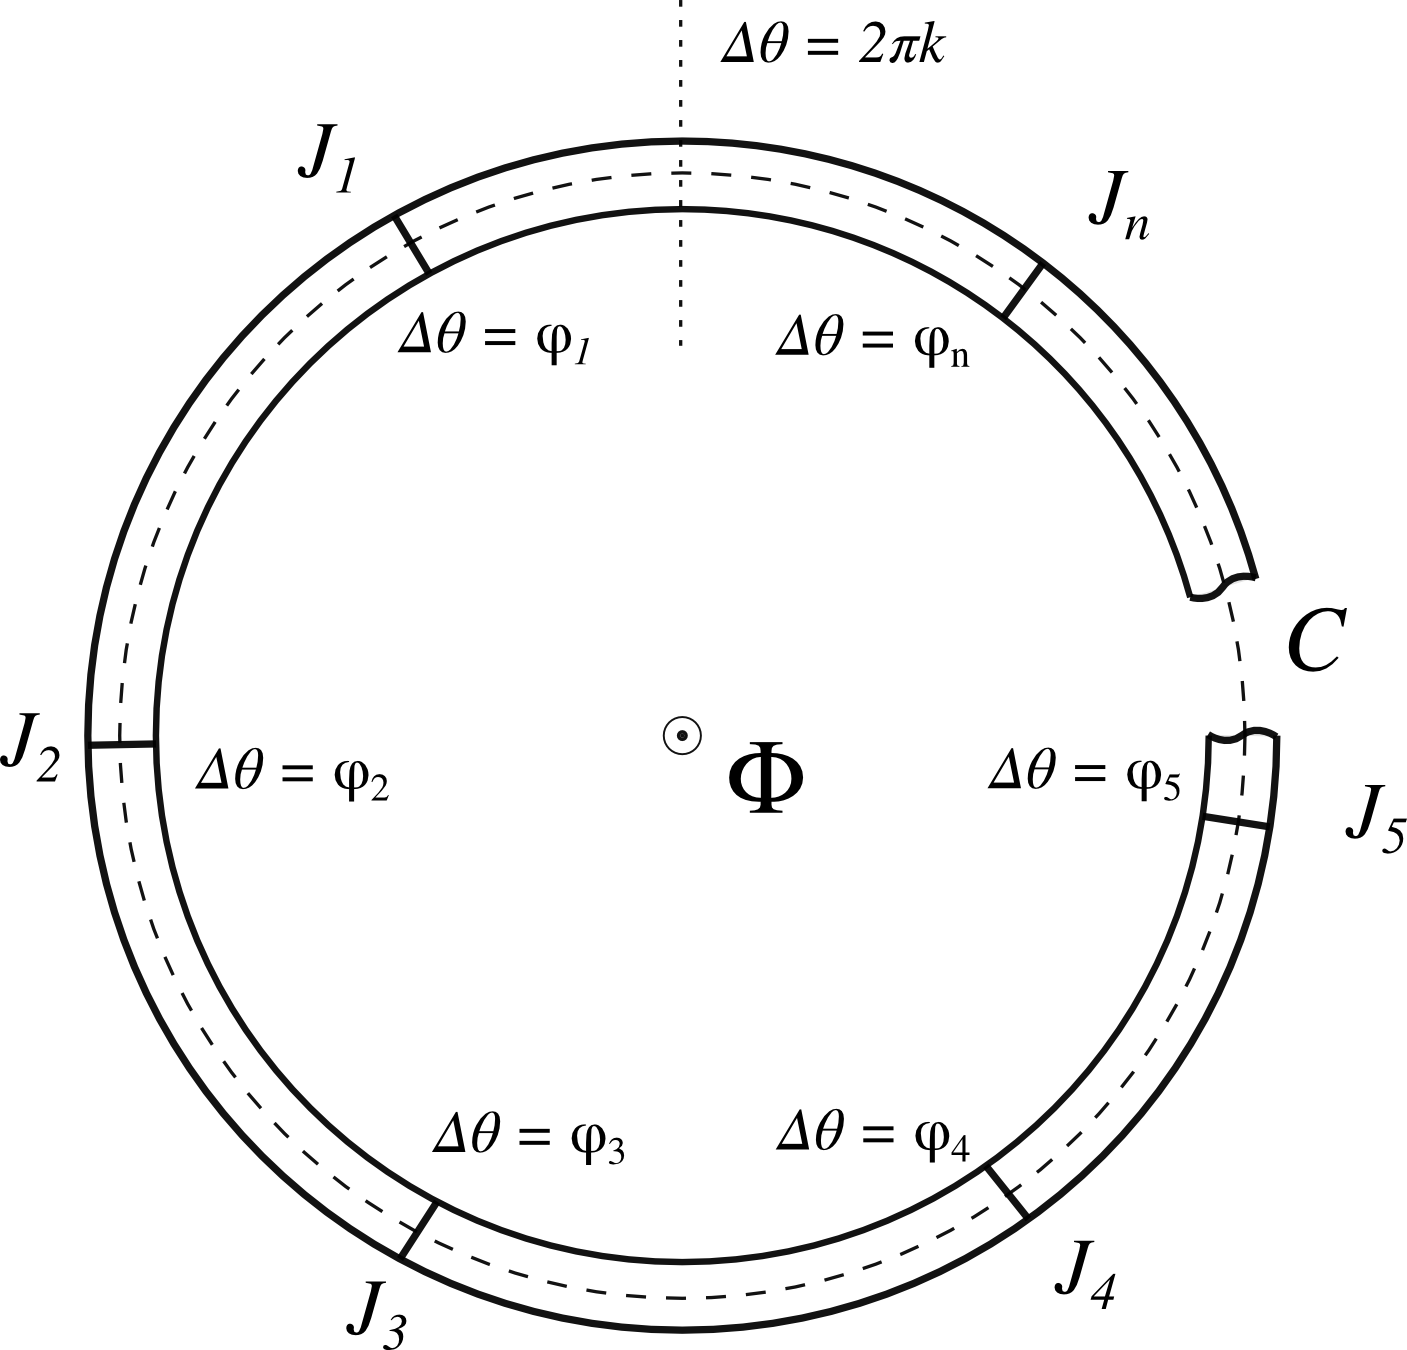
\includegraphics[width=0.5\linewidth]{Pictures/ring.png}
\caption{К выводу фазо-потокового соотношения. Пунктиром обозначен контур интегрирования C. Через $\varphi_i$ обозначены скачки фаз на джозефсоновских контактах, а точками - место разрешенного накопления фазы при полном обходе вокруг кольца $2\pi k,\ k\in\mathcal{Z}$.}
\label{fig:ring}
\end{figure}

Таким образом, получено фазо-потоковое соотношение. Видно, что в случае отсутствия в кольце джозефсоновских переходов полученное уравнение (\ref{eq:phsflx}) опишет равенство магнитного потока $\Phi$, проходящего через сверхпроводящее кольцо, целому числу  k квантов потока $\Phi_0$, обосновывая определение этой константы в (\ref{eq:lond2}).


\section{Теория изолированного Flux-кубита}
Flux-кубит, или потоковый трехконтактный сверхпроводящий кубит, был предложен впервые в 1999 году\cite{Orlando1999} и представляет собой сверхпроводящий контур, прерванный в трех местах джозефсоновскими переходами (\autoref{fig:qubit}), два из которых одинаковы, а третий отличается по площади в $\alpha$ раз. Под \textit{изолированным} в данном разделе понимается одиночный кубит, не взаимодействующий с окружением ни диссипативным, ни консервативным образом. Единственным внешним фактором является при таком рассмотрении постоянное магнитное поле, проходящее через контур.

\begin{figure}
\centering
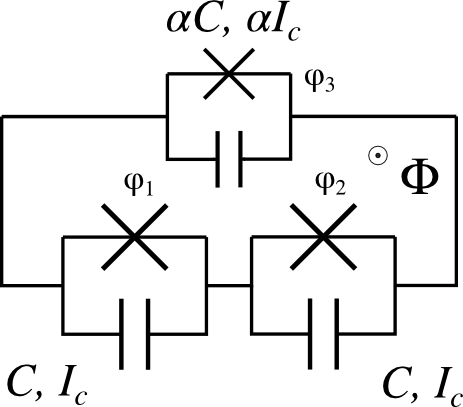
\includegraphics[width=0.4\textwidth]{Pictures/qubit}
\caption{Принципиальная схема Flux-кубита в рамках RCSJ-модели. Два из трех переходов по площади одинаковы, площадь третьего по сравнению с ними в $\alpha$ раз отличается (параметры отличаются в то же число раз согласно формулам для емкости конденсатора и (\ref{eq:Ic})). $\Phi$ -- поток, пронизывающий контур. Резисторы не изображены, так как рабочий ток переходов меньше $I_c$.}
\label{fig:qubit}
\end{figure}

\subsection{Построение гамильтониана}
Для того, чтобы провести квантово-механическое рассмотрение кубита, требуется записать его гамильтониан. Для этого прежде всего нужно понять, какими независимыми степенями свободы он обладает. Вообще говоря, состояние одиночного джозефсоновского перехода, в силу того, что в параллельном соединении RCSJ-модели $U = \frac{\hbar}{2e}\dot\varphi$, целиком описывается своей разностью фаз. Для трех невзаимодействующих переходов таких разностей будет три, и их и следует выбрать в качестве обобщенных координат системы. Однако в случае замкнутого контура дополнительно накладывается фазо-потоковое соотношение (\ref{eq:phsflx}):
\begin{equation}
\varphi_1 + \varphi_2 + \varphi_3 = 2\pi\left(\frac{\Phi}{\Phi_0} - k\right),\ k\in \mathcal{Z}.
\label{eq:qubit_phsflx}
\end{equation}
Таким образом, в контуре на \autoref{fig:qubit} остаются независимыми только две разности фаз из трех. Введя их в качестве обобщенных координат, можно понять, что является аналогом кинетической, а что -- потенциальной энергии системы. В уравнениях (\ref{eq:JJenrj1})-(\ref{eq:JJenrj2}) энергия перехода зависит непосредственно от $\varphi$, а емкостная от $\dot \varphi$. Таким образом, переход запасает потенциальную, а емкость кинетическую энергию. Энергия магнитного поля, возникающего при течении тока в кольце, считается малой в силу малости геометрической индуктивности кубита по сравнению с джозефсоновской индуктивностью переходов, а поток $\Phi = \Phi_{ext}$ (подробное описание данной процедуры см. в статье \cite{Robertson2006}). Теперь можно записать лагранжиан системы, используя все те же уравнения (\ref{eq:JJenrj1})-(\ref{eq:JJenrj2}) и выражая разность фаз $\varphi_3$ отличающегося перехода через разности фаз $\varphi_1$ и $\varphi_2$ одинаковых переходов при помощи (\ref{eq:qubit_phsflx}):
\begin{gather*}
\mathcal{L} = \mathcal{T}-\mathcal{U}, \\
\mathcal{T} = E_{cap} =\frac{1}{2}\sum_{i=1}^3 C_i V_i^2 = \frac{1}{2} \left(\frac{\Phi_0}{2\pi}\right)^2 \left[C(\dot \varphi_1)^2 + \alpha C \left(\dot \varphi_1 + \dot\varphi_2\right)^2 + C(\dot \varphi_2)^2\right] \\
= \frac{1}{2}\left(\frac{\Phi_0}{2\pi}\right)^2 \left(\begin{matrix}
\dot\varphi_1 &\dot\varphi_2
\end{matrix}\right) C \left(\begin{matrix}
1+\alpha & \alpha \\
\alpha & 1+\alpha
\end{matrix}
\right)
\left(\begin{matrix}
\dot\varphi_1 \\
\dot\varphi_2
\end{matrix}\right),\\
\mathcal{U} = E_{ind} = E_J\left[2+\alpha + \cos\varphi_1 + \cos\varphi_2 + \alpha \cos\left(2\pi\frac{\Phi}{\Phi_0} - \varphi_1 - \varphi_2 \right)\right].
\end{gather*}
Строить гамильтониан системы из такого лагранжиана не очень удобно, поэтому предварительно произведем замену координат $\displaystyle \phi = \frac{\varphi_1 + \varphi_2}{2},\ \theta = \frac{\varphi_1 - \varphi_2}{2}$:
\begin{gather}
\mathcal{T}  \overset {\varphi_1, \varphi_2 \rightarrow \phi, \theta}{=}
C\left(\frac{\Phi_0}{2\pi}\right)^2 (\begin{matrix}
\dot \phi & \dot \theta
\end{matrix})
\left(\begin{matrix}
1+2\alpha & 0\\
0 & 1
\end{matrix}
\right)
\left(\begin{matrix}
\dot \phi \\ \dot \theta
\end{matrix}\right), \notag
\\
\mathcal{U} \overset {\varphi_1, \varphi_2 \rightarrow \phi, \theta}{=} E_J\left[2+\alpha - 2\cos(\phi)\cos(\theta) - \alpha\cos\left(2\pi\frac{\Phi}{\Phi_0} -2\phi\right)\right].
\label{eq:U_qb}
\end{gather}
Теперь, стандартным образом вводя обобщенный импульс 
$\displaystyle \mathbf{p}^T = \left(\begin{matrix}p_\phi & p_\theta\end{matrix}\right) = \left(\begin{matrix}\frac{\partial\mathcal{L}}{\partial\dot\phi} & \frac{\partial\mathcal{L}}{\partial\dot\theta}\end{matrix}\right)$ и производя преобразование Лежандра, получим итоговый гамильтониан системы:
\begin{gather*}
\mathcal{H} = \frac{p_\phi^2}{2M_\phi} + \frac{p_\theta^2}{2M_\theta}+ E_J\left[2+\alpha - 2\cos(\phi)\cos(\theta) - \alpha\cos\left(2\pi\frac{\Phi}{\Phi_0} -2\phi\right)\right], \\
M_\phi = 2C\left(\frac{\Phi_0}{2\pi}\right)^2(1+2\alpha),\ M_\theta = 2C\left(\frac{\Phi_0}{2\pi}\right)^2.
\end{gather*}
Далее, осуществляя переход к операторному виду квантовой механики, можно получить оператор Гамильтона для сверхпроводящего потокового кубита в терминах исключительно $E_C$ и $E_J$:
\begin{gather}
\hat{\mathcal{H}} = E_C\left[-\frac{1}{2(1 + 2\alpha)}\frac{\partial^2}{\partial\phi^2} 
- \frac{1}{2}\frac{\partial^2}{\partial\theta^2}\right] + \notag \\+ E_J\left[2+\alpha - 2\cos(\phi)\cos(\theta) - \alpha\cos\left(2\pi\frac{\Phi}{\Phi_0} -2\phi \right)\right].
\label{eq:hamiltonian}
\end{gather}

\subsection{Квантово-механический анализ}

\begin{figure}[!p]
\begingroup
\captionsetup[subfigure]{width=0.95\textwidth}
\centering
\begin{subfigure}[t]{0.49\linewidth}
\centering
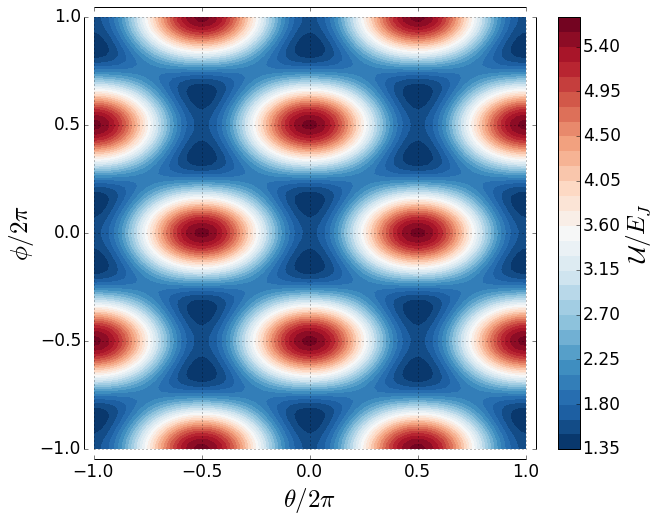
\includegraphics[height = .8\textwidth]{Pictures/qubit_potential}
\caption{Трехмерное изображение потенциала при $\Phi = \Phi_0/2,\ \alpha=0.8$. Можно видеть $2\pi$-периодическую центрированную квадратную решетку с базисом из двойных ям.}
\label{fig:U3d}
\end{subfigure}~
\begin{subfigure}[t]{0.49\linewidth}
\centering
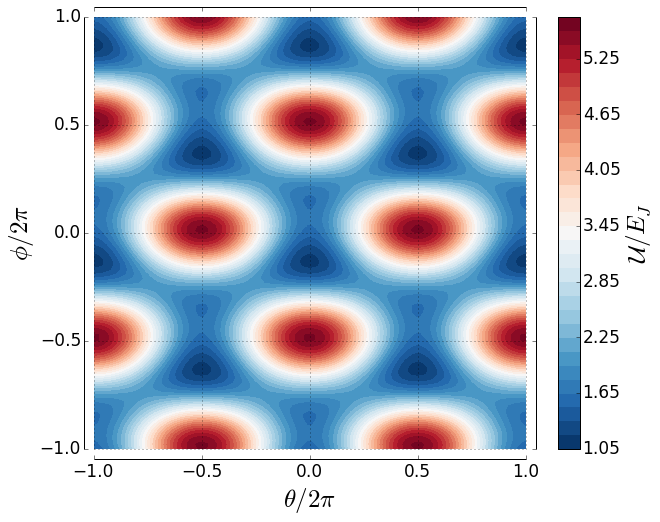
\includegraphics[height = .8\textwidth]{Pictures/qubit_potential2}
\caption{При отклонении потока от $\Phi_0/2$ появляется перекос внутри двойных ям, одна половина становится глубже, а другая мельче в зависимости от знака отклонения $\Delta\Phi$. Здесь $\Delta\Phi=-0.05\Phi_0,\ \alpha=0.8$}
\label{fig:U3d2}
\end{subfigure}
\begin{subfigure}[t]{0.49\linewidth}
\centering
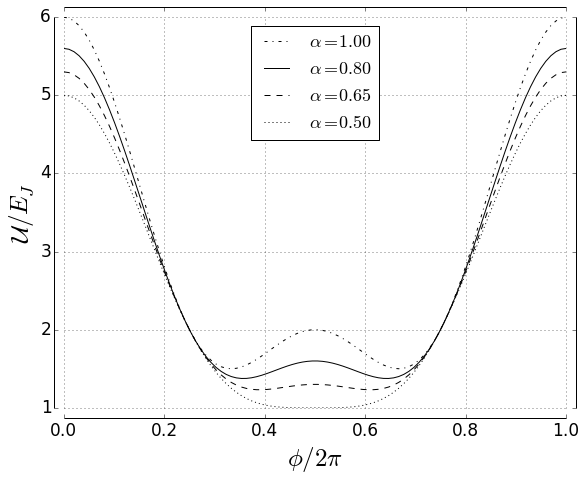
\includegraphics[height = 0.8\textwidth]{Pictures/qubit_potential_cut}
\caption{Срез потенциала при $\Phi = \Phi_0/2$ по направлению $\theta = \pi$ (барьер внутри ям) в зависимости от $\alpha$. При $\alpha = 0.5$ этот барьер пропадает, при $\alpha=1$ он сравнивается с барьером между ямами (см. (\subref{fig:U_cut2})).}
\label{fig:U_cut}\quad
\end{subfigure}
\begin{subfigure}[t]{0.49\linewidth}
\centering
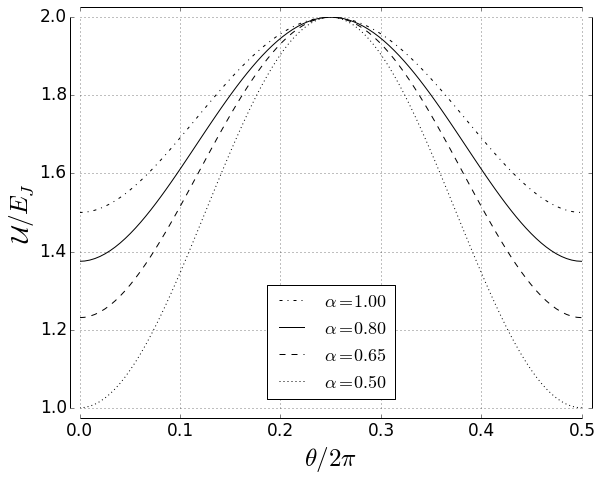
\includegraphics[height = 0.8\textwidth]{Pictures/qubit_potential_cut2}
\caption{Срез потенциала при $\Phi = \Phi_0/2$ по направлению $\phi = \left(1 - \frac{2}{\pi}\arccos
\frac{1}{2\alpha}\right)\theta+\arccos\frac{1}{2\alpha}$ (барьер между ямами) в зависимости от $\alpha$. Здесь крайние точки отвечают минимумам $\mathcal{U}$ при $\theta=0\ (\pi),\ \phi=\arccos
\frac{1}{2\alpha}\ \left(\pi - \arccos\frac{1}{2\alpha}\right)$.}
\label{fig:U_cut2}
\end{subfigure}
\endgroup
\caption{Графическое изображение периодического потенциала Flux-кубита в зависимости от относительного размера отличающегося перехода $\alpha$ и пронизывающего потока $\Phi$.}
\label{fig:U_fq}
\end{figure} 

\paragraph{Анализ потенциала.} Прежде всего рассмотрим потенциал $\mathcal{U}(\phi, \theta)$. На \autoref{fig:U_fq} представлены графики, демонстрирующие его структуру в случае $\Phi = \Phi_0/2$, или в так называемой \textit{точке вырождения} по потоку. На \autoref{fig:U_fq}~(\subref{fig:U3d}) можно видеть, что потенциал $2\pi$-периодичен по каждой из переменных $\phi$ и $\theta$ и представляет собой бесконечную центрированную квадратную решетку с базисом из симметричных двойных ям, отделенных друг от друга диагональными барьерами. Каждая их ям, в свою очередь, делится на две части меньшим барьером. Его высота, как видно из \autoref{fig:U_fq}~(\subref{fig:U_cut}), определяется параметром $\alpha$. Для того, чтобы структура оставалась подобной изображенной на \autoref{fig:U_fq}~(\subref{fig:U3d}), требуется, чтобы $\alpha\in(0.5,\ 1)$: при нарушении этого условия либо совсем пропадает внутренний барьер, либо внешний барьер сравнивается с внутренним по высоте, и ямы перестают быть качественно отделены друг от друга (\autoref{fig:U_fq}~(\subref{fig:U_cut2})). Минимумы $\mathcal{U}$ находятся в точках $\theta=\pi k,\ \phi=\pm\arccos\frac{1}{2\alpha}+\pi \frac{n}{2},\ k,\ n\in\mathcal{Z}$, причем в точке вырождения все минимумы имеют одинаковую энергию, а при отходе от нее в зависимости от знака отклонения одна половина двойных ям становится мельче, а другая глубже, и вырождение внутри каждой ямы снимается (\autoref{fig:U_fq}~(\subref{fig:U3d2})). 

\begin{figure}[!p]
\begingroup
\captionsetup[subfigure]{width=\textwidth}
\centering
\begin{subfigure}[t]{0.75\linewidth}
\centering
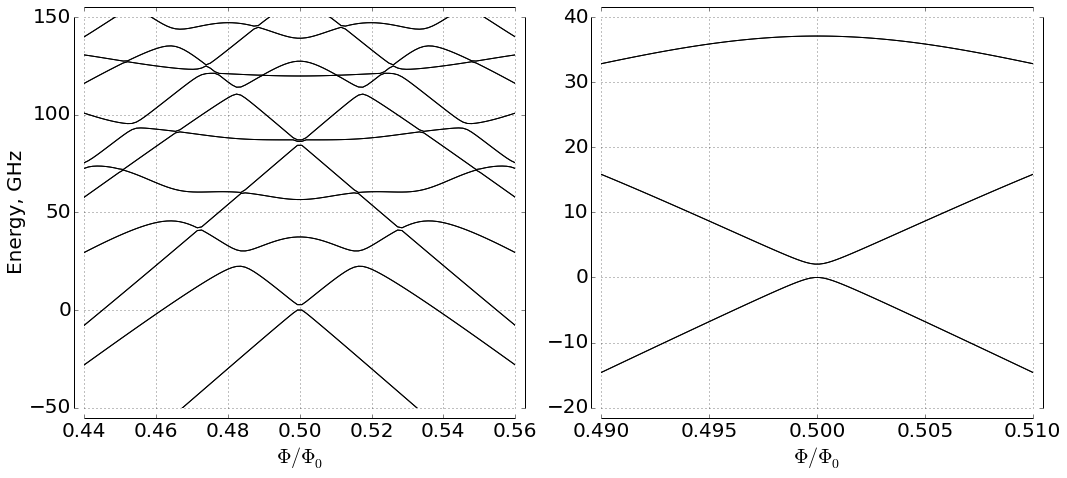
\includegraphics[width = \textwidth]{Pictures/qubit_levels}
\caption{Уровни энергии в зависимости от внешнего поля. Каждая линия на рисунке на самом деле является двойной (подробности см. в тексте).}
\label{fig:levels}
\end{subfigure}

\begin{subfigure}[t]{0.8\linewidth}
\centering
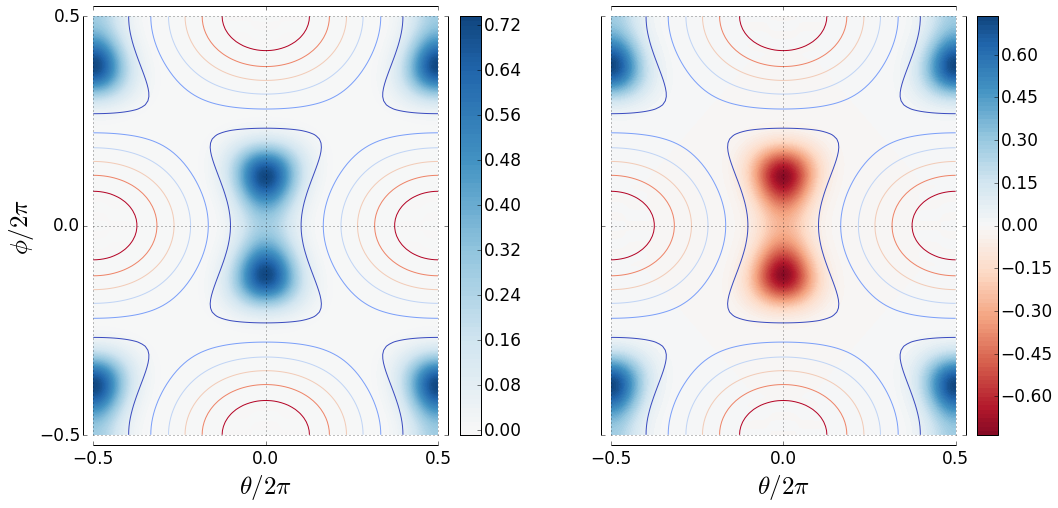
\includegraphics[width = \textwidth]{Pictures/wfs01}
\caption{Граничные по квазиимпульсу состояния нулевой зоны (``$\ket{g}$-состояния'') в точке вырождения. Внутри ям волновая функция четная.}
\label{fig:wfs01}
\end{subfigure}

\begin{subfigure}[t]{0.8\linewidth}
\centering
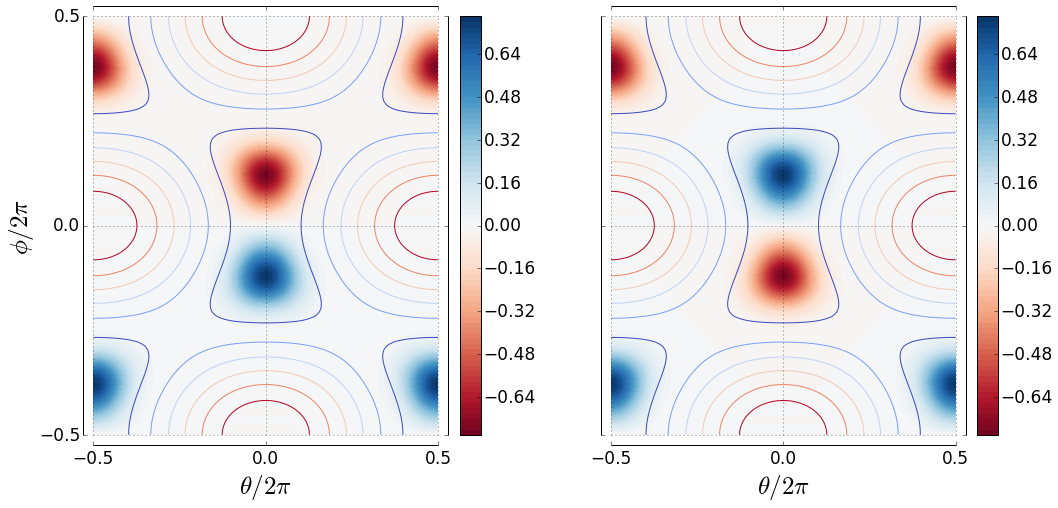
\includegraphics[width = \textwidth]{Pictures/wfs23}
\caption{Граничные по квазиимпульсу состояния первой зоны (``$\ket{e}$-состояния'') в точке вырождения. Внутри ям волновая функция нечетная.}
\label{fig:wfs23}
\end{subfigure}

\endgroup
\caption{Результаты численного решения стационарного уравнения Шредингера с параметрами $\alpha=0.7,\ E_J  = 30E_C = 400\ \text{GHz}$. Цветом обозначено значение волновой функции, нормированной на единицу в периоде потенциала.}
\label{fig:numerical_res}
\end{figure} 

\paragraph{Стационарные состояния.} Прежде, чем начинать поиск стационарных состояний для гамильтониана (\ref{eq:hamiltonian}), важно не упустить смысл происходящего. Строго говоря, в силу того, что потенциал (\ref{eq:U_qb}) является периодическим, решениями уравнения Шредингера будут являться \textit{блоховские функции}, а спектр энергий будет иметь зонную структуру. Таким образом, в приближении нулевой индуктивности Flux-кубит представляет собой модель частицы в идеальной периодической решетке двумерного твердого тела. В реальности, однако, энергетический спектр все же является дискретным из-за квадратичной по фазам индуктивной энергии\cite{Robertson2006}, с пиками числа уровней в областях бывших зон. 

Оставаясь в рамках приближения нулевой индуктивности, для аналитического решения задачи можно использовать модель сильной связи для центрированной решетки с базисом, однако мы будем рассматривать численный вариант -- метод, изложенный в работе\cite{Johansson}. В условиях $2\pi$-периодичности и действительности потенциала и искомой волновой функции можно разложить в ряд Фурье, ограничиваясь $2N+1$ начальными слагаемыми, уравнение Шредингера с гамильтонианом (\ref{eq:hamiltonian}), что после определенных преобразований сведет задачу к поиску собственных значений и векторов матрицы размером $(2N+1)^2$ на $(2N+1)^2$. Результаты такого вычисления для $N=20$ представлены на \autoref{fig:numerical_res}. Вычисленный спектр энергий (\autoref{fig:numerical_res}~(\subref{fig:levels})) состоит из дублетов (на рисунке они сливаются в синглеты), причем расщепление в дублетах обусловлено разными периодическими конфигурациями волновой функции при фиксированной четности ее внутри ям, а расстояния между дублетами изменением четности внутри ям. Такая структура спектра возникает по причине того, что в силу использованных предположений о волновой функции машинный метод ``вылавливает'' из каждой энергетической зоны лишь граничные состояния, так как только они обладают подходящими свойствами! Действительно, по теореме Блоха $\psi(r) = e^{ikR}\psi(r)$, для граничных квазиимпульсов $k = 0$  и $k = K/2$ ($K$-вектор обратной решетки) выполнено соответственно $\psi(r+R) = \psi(r)$ и $\psi(r+R)=-\psi(r)$, что и наблюдается на парах \autoref{fig:numerical_res}~(\subref{fig:wfs01}) и \autoref{fig:numerical_res}~(\subref{fig:wfs23}). Четные конфигурации волновой функции имеют меньшую рассчитанную энергию, а нечетные большую, в соответствии с вышесказанным.

В зависимости от поля спектр ведет себя, как показано на \autoref{fig:numerical_res}~(\subref{fig:levels}), неравномерно: в окрестности $\Phi_0/2$ четные зоны сдвигаются вниз, нечетные вверх, а на большем удалении магнитного потока от полкванта картина вообще теряет порядок из-за значительного числа квазипересечений. На \autoref{fig:numerical_res}~(\subref{fig:wfs01}) и (\subref{fig:wfs23}) изображены соответственно нулевое и первое дублетные состояния в точке вырождения.  Далее мы будем пренебрегать тем, что первые две зоны отличны от дискретных уровней, так как расщепления внутри них примерно в $10^5$ раз меньше, чем расстояния между ними, и назовем верхнюю по энергии зону ``$\ket{e}$-состоянием'', а нижнюю ``$\ket{g}$-состоянием''.

\paragraph{Двухуровневое приближение.} Следующим шагом будет приведение системы к двум нижним состояниям, пренебрегая всеми остальными. Это оправданно, так как третья зона в окрестности точки вырождения лежит гораздо выше (почти в 20 раз) по энергии, чем состояние $\ket{e}$ . Теперь, используя метод сильной связи в двойной яме, рассчитаем зависимость расщепления уровней $\ket{g}$ и $\ket{e}$ от $\Phi$. Разобьем яму на два потенциала $\mathcal{U}_1$ и $\mathcal{U}_2$, так, что их сумма даст исходный потенциал ямы, а не равными нулю они окажутся только в области соответствующих полуям. Для каждого из этих двух потенциалов можно найти основные состояния, которые мы обозначим $\ket{1, g}$ и $\ket{2, g}$. Основное состояния для уравнения с потенциалом $\mathcal{U}_1+\mathcal{U}_2$ в предположении о малом перекрытии потенциалов и волновых функций отдельных ям можно искать в виде $\ket{g} = a\ket{1, g} + b\ket{2, g}$. Также мы получим сразу и $\ket{e}$ в качестве второго решения задачи. Итак, записывая полный гамильтониан, действуя им на выбранного вида функцию $\ket{g}$ и умножая слева сначала на $\bra{1, g}$, а потом на $\bra{2, g}$, получим следующую систему уравнений:
\begin{align*}
\left(\begin{matrix}
E_{1g}+U_2^{1g1g} & E_{1g}\braket{1,g}{2,g} + U_2^{1g2g}\\ 
E_{2g}\braket{2,g}{1,g} + U_1^{2g1g} & E_{2g} + U_1^{2g2g}
\end{matrix}\right) 
\left(\begin{matrix}
a \\b 
\end{matrix}\right) = 
E\left(\begin{matrix}
1 & \braket{1,g}{2,g} \\
\braket{2,g}{1,g} & 1
\end{matrix}\right)
\left(\begin{matrix}
a \\b 
\end{matrix}\right),
\end{align*}
где верхними индексами обозначены соответствующие матричные элементы потенциалов $U$, $E_{1g}, E_{2g}$ -- энергии основных состояний ям, $E$ -- искомое собственное значение полного гамильтониана. Далее, пренебрежем диагональными матричными элементами потенциалов, так как здесь они берутся по волновым функциям противоположной половины ямы, а также неортогональностью $\ket{1, g}$ и $\ket{2, g}$ (они также локализованы в разных ямах). Тогда уравнение значительно упростится:
\begin{align*}
\left(\begin{matrix}
E_{1g} &  U_2^{1g2g}\\ 
U_1^{2g1g} & E_{2g}
\end{matrix}\right) 
\left(\begin{matrix}
a \\b 
\end{matrix}\right) = 
E
\left(\begin{matrix}
a \\b 
\end{matrix}\right).
\end{align*}
Следующим приближением будет пренебрежение различием в недиагональных элементах, так как при малых отклонениях $\Phi$ деформации около дна ям незначительны, и можно считать, что формы волновых функций и потенциалов остаются прежними, а меняются лишь энергии основных состояний из-за перекоса ям. Переобозначая элементы матрицы и смещая собственные значения на постоянную величину, получаем сокращенный гамильтониан следующего вида:
\begin{gather}
\mathcal{\hat H} = \frac{\delta}{2} \hat\sigma_z + \frac{\Delta}{2} \hat \sigma_x \Leftrightarrow \frac{\delta}{2} \hat\sigma_x + \frac{\Delta}{2} \hat \sigma_z \\ 
\text{(с точностью до выбора базиса)} \notag
\label{eq:trunc_hamiltonian}
\end{gather}
где $\Delta = 2 U_1^{2g1g} \approx 2U_2^{1g2g}$ -- минимальное расщепление по энергии, $\delta = |E_{1g} - E_{2g}|$ -- сдвиг энергий основных состояний ям в зависимости от поля. После дифференцирования потенциала можно получить, что сдвиг минимумов по энергии, а, следовательно, и $\delta$, будут пропорциональны $\Phi - \Phi_0/2$.

Сокращенный гамильтониан \eqref{eq:trunc_hamiltonian} можно просто привести к диагональному виду. Его собственные значения и их разность будут зависеть от $\delta$ следующим образом:
\begin{equation}
E_{g, e} = \pm \frac{1}{2}\sqrt{\Delta^2 + \delta^2},\
\Delta E = h \nu_q = \sqrt{\Delta^2 + \delta^2},
\end{equation}
где $\nu_q$ -- это экспериментально наблюдаемая частота перехода между кубитными уровнями. Легко построить зависимость этой частоты от приложенного поля -- это гипербола.

Главным обоснованием сделанных приближений является точный численный результат \autoref{fig:numerical_res}~(\subref{fig:levels}) для двух нижних состояний, который так же дает гиперболическую зависимость.

\section{Взаимодействие кубита с окружающей средой}

Переход от замкнутых квантовых систем, эволюция которых подчинена нестационарному уравнению Шредингера и состояние которых в каждый момент времени точно известно, к так называемым \textit{открытым}, т.е. незамкнутым, квантовым системам всегда сопряжен с трудностями. Это связано с тем, что для описания таких систем в идеале требовалось бы найти закон эволюции Вселенной, а затем исключить из рассмотрения все ее степени свободы, не касающиеся представляющей интерес области. Эта формулировка является, конечно, довольно туманной в отношении Вселенной, но что вообще такое Вселенная? В силу отсутствия однозначного ответа на данный вопрос в качестве ``вселенной'' часто выбирают что-то простое, такое, что в определенных приближениях можно описать математически -- и получают результаты, согласующиеся с экспериментом\cite{bishop2009}. Далее будет описана такая процедура и соответствующий математический аппарат.

\subsection{Матрица плотности}

Матрица плотности -- это обобщение вектора состояния на системы, точное состояние которых неизвестно. Матрицы плотности подразделяются на \textit{чистые} и \textit{смешанные}: первые эквивалентны обычной волновой функции, вторые же определяют распределение вероятности на волновых функциях. Рассмотрим две ситуации:
\begin{enumerate}
\item Система находится в суперпозиции состояний из какого-либо набора $\ket{a} = \sum_k c_k \ket{k}$. Тогда матрица плотности является чистой и записывается следующим образом: 
\[ \hat \rho_a = \ket{a}\bra{a} = \sum_{k,n}c_k c_n^* \ket{k}\bra{n}.\]
\item Система находится в каком-то одном из состояний $\ket{k}$ с вероятностью $c_k^2$. Тогда матрица плотности является смешанной и записывается теперь иначе:
\[ 
\hat \rho_a = \sum_k c_k^2 \ket{k}\bra{k}.
\]
\end{enumerate}
В чем удобство таких определений? Для ответа на этот вопрос рассмотрим значение произвольной наблюдаемой с оператором $\hat Q$. В первом случае, из определения:
\[
Q = \bra{a}\hat Q\ket{a} = \sum_{k,n} c_k c_n^* \bra{n}\hat Q\ket{k}\ \equiv \sum_i \sum_{k,n} c_k c_n^* \braket{i}{k} \bra{n} \hat Q \ket{i} \overset{def}{=}\Tr{\hat \rho_a \hat Q}. 
\]
Во втором случае, из определения и квантового, и статистического среднего, а также приема, примененного выше, для каждого вероятного состояния:
\[
Q = \sum_k Q_k p_k = \sum_k \Tr{ \ket{k}\bra{k} \hat Q} p_k \equiv \Tr{\hat \rho_a \hat Q}. 
\]
Таким образом, через матрицу плотности мы получаем единое определение среднего значения оператора, имеющего смысл как для статистического, так и для простого квантового случая. Также просто показывается, что обе матрицы плотности удовлетворяют одному и тому же уравнению Лиувилля-фон-Неймана: 
\[ 
i\hbar \frac{\partial}{\partial t} \hat \rho = [\mathcal{\hat H}, \hat \rho].
\]

В качестве примера того, как матрица плотности может помочь при описании открытых систем, рассмотрим два кубита, находящихся в \textit{перепутанном} состоянии, когда невозможно представить их общее состояние как тензорное произведение векторов состояний кубитов по отдельности. Такое состояние -- это, например, 
\[
\ket{\Psi^+} = \frac{1}{\sqrt{2}}(\ket{\uparrow}_A\otimes\ket{\downarrow}_B+\ket{\downarrow}_A\otimes\ket{\uparrow}_B).
\]
Соответствующая матрица плотности:
\[ 
\hat \rho_{\Psi^+} = \frac{1}{2} \rbrkt{\begin{matrix}
0&0&0&0\\
0&1&1&0\\
0&1&1&0\\
0&0&0&0
\end{matrix} }.
\]
Каждый из кубитов в примере является, по сути, открытой системой, которую требуется описать. Для этого вводится понятие \textit{сокращенной матрицы плотности} и операция взятия \textit{частичного следа} для системы двух подсистем:
\[
\hat \rho_A = \pTr{B}{\hat \rho_{AB}} \overset{def}{=} \sum_i \bra{i}_B \hat \rho_{AB} \ket{i}_B \ \Leftrightarrow \ [\hat \rho_A]_{n, m} = \sum_i \bra{n}_A \! \otimes\! \bra{i}_B\ \hat \rho_{AB}\ \ket{i}_B\!\otimes\! \ket{m}_A,
\] 
где суммирование ведется по базису подсистемы B (второе выражение показывает, как суммировать по состояниям композитного базиса $\mathcal{A}\otimes \mathcal{B}$). Для каждого из двух кубитов системы в состоянии $\ket{\Psi^+}$ такое вычисление даст $\hat \rho_{A,B} = \mathbbm{\hat 1}_{A, B}/2$ -- матрица плотности каждого из них смешанная и дает 50\%-ую вероятность быть в одном из двух состояний. Таким образом, зная все о перепутанной системе, мы не имеем достоверной информации о ее частях.

\subsection{Уравнение эволюции в форме Линдблада}

Процедура сокращения матрицы плотности, проведенная с двумя кубитами и их общим стационарным состоянием, применяется и в нестационарном случае для получения уравнения эволюции подсистемы (master equation)\cite{carmichael1999}. Исходный гамильтониан включает систему, ее окружение и их взаимодействие:
\begin{gather}
\mathcal{\hat H}_{se} = \mathcal{\hat H}_s \otimes \mathbbm{\hat 1}_e + \mathbbm{\hat 1}_s \otimes \mathcal{\hat H}_e + \mathcal{\hat H}_i. 
\label{eq:H_se}
\\
i\hbar \frac{\partial}{\partial t} \hat \rho_{se} = [\mathcal{\hat H}_{se}, \hat \rho_{se}]
\label{eq:se_se}
\end{gather}
Теперь обозначим приближения, которые используются для получения сокращенного уравнения эволюции (хорошее обсуждение их соответствия реальности см. в работе \cite{rivas2010}):
\begin{enumerate}
\item \textbf{Модель окружения.} В качестве модели внешней среды обычно используется бозе-термостат, т.е. $  \mathcal{\hat H}_e = \sum_k \hbar \omega_k \hat a_k^\dag \hat a_k$ в \eqref{eq:H_se}, а взаимодействие $\mathcal{\hat H}_i$ однобозонным и слабым.
\item \textbf{Борновское приближение.} При решении уравнения \eqref{eq:se_se} мы ищем матрицу плотности системы в виде $\hat \rho_{se}(t) = \hat \rho_{s}(t) \otimes \hat \rho_{e}^0$, тем самым пренебрегая изменением состояния термостата $\displaystyle \hat \rho_{e}^0 = \exp\rbrkt{\mathcal{\hat H}_{e}}/\Tr{\exp\rbrkt{\mathcal{\hat H}_e}}$.
\item \textbf{Приближение Маркова.} Эволюция $\hat \rho_{s}$ после момента t определяется только ее значением в этот момент и не зависит от прошлых значений. По-другому это формулируется как отсутствие памяти у термостата. 
\end{enumerate}
В условиях выбранных приближений можно путем достаточно громоздких преобразований получить уравнение динамики подсистемы. Его часть, ведущая к отличиям от стандартной унитарной эволюции, окажется представимой в \textit{форме Линдблада}, и, в итоге, искомое уравнение будет иметь следующий вид:

\begin{gather}
i\hbar \frac{\partial}{\partial t}\hat \rho_s = \sbrkt{\mathcal{\hat H}_s, \hat \rho_s} +
\sum_k \Gamma_k \rbrkt{\mathcal{\hat O}_k \hat \rho_s \mathcal{\hat O}_k^\dag - \frac{1}{2} \left\{ \mathcal{\hat O}_k^\dag \mathcal{\hat O}_k, \hat \rho_s \right\} } \\
\overset{def}{=} \sbrkt{\mathcal{\hat H}_s, \hat \rho_s} + \sum_k \Gamma_k \mathcal{D}\sbrkt{\mathcal{\hat O}_k}\hat \rho_s.
\label{eq:gen_lind}
\end{gather}
$\mathcal{\hat D}$ - линдбладовский супероператор. Коэффициенты $\Gamma_k$, определяющие скорость распада, и операторы $\mathcal{\hat O}_k$, определяющие каналы распада, выводятся\cite{carmichael1999} для каждой конкретной модели, для каждого гамильтониана \eqref{eq:H_se}, однако вид \eqref{eq:gen_lind} сохраняется (это можно показать в рамках теории групп\cite{lindblad1976}). 

\subsection{Релаксация}

Для получения диссипатора, отвечающего за передачу энергии кубита внешнему бозе-полю, используется следующий модельный гамильтониан:

\begin{equation}
\mathcal{\hat H}_{se} = \frac{\hbar \omega_q}{2} \hat \sigma_z \otimes \mathbbm{\hat 1}_e + \mathbbm{\hat 1}_q \otimes  \sum_k \hbar \omega_k \hat a_k^\dag \hat a_k  + \sum_k g_k \rbrkt{\hat \sigma^-\otimes \hat a_k^\dag +  \hat \sigma^+ \otimes \hat a_k},
\label{eq:rel_model}
\end{equation}
где $\omega_q, \omega_k$ -- энергии кубита и мод, $\hat \sigma^{\pm}$ -- повышающий и понижающий операторы кубита, $\hat \sigma^+ = \hat{\sigma}^{-^\dag} = \ket{e}\bra{g}$, а $g_k$ -- константы связи кубита с внешним полем. Последняя часть возникает из взаимодействия квантованного поля каждой моды, которое пропорционально $\hat a_k^+ + \hat a_k$, с кубитом (через оператор $\hat \sigma_x = \hat \sigma^-+  \hat \sigma^+ $, см. \eqref{eq:trunc_hamiltonian}) в первом порядке теории возмущений, т.е. $\mathcal{\hat H}_{i_k} \propto \rbrkt{\sigma^-+  \hat \sigma^+}\otimes\rbrkt{\hat a_k^+ + \hat a_k}\overset{\mathbb{I}\, ord.}{\rightarrow} (\hat \sigma^-\otimes \hat a_k^\dag +  \hat \sigma^+ \otimes \hat a_k)$. Это оправданно, так как мы полагаем связи, т.е. $g_k$, малыми. Исходя из такой модели при $T \approx 0$ получаем\cite{carmichael1999} следующее уравнение эволюции:
\begin{equation}
i \hbar \frac{\partial}{\partial t}\hat \rho_q = \sbrkt{\mathcal{\hat H}_q, \hat \rho_q} +
\gamma (\hat \sigma^- \hat \rho_q \hat \sigma^+ - \frac{1}{2} \left\{ \hat\sigma^+\hat\sigma^-, \hat \rho_q \right\} ),
\end{equation}
где $\gamma$ получается в процессе вычисления из \eqref{eq:rel_model}, однако на практике подгоняется к экспериментальным данным. Динамику данного уравнения мы обсудим несколько позже.

\subsection{Дефазировка}

Более тонкий эффект получится, если мы будем рассматривать другую модель, выбрав следующий вид гамильтониана \eqref{eq:H_se}\cite{carmichael1999}:

\begin{align}
\mathcal{\hat H}_{q} &= \frac{\hbar \omega_q}{2} \hat \sigma_z \notag \\
\mathcal{\hat H}_{e} &= \sum_k \hbar \omega_{1k} \hat a_{1k}^\dag \hat a_{1k}  +\sum_k \hbar \omega_{2k} \hat a_{2k}^\dag \hat a_{2k} 
\label{eq:deph_model}
\\
\mathcal{\hat H}_i &= \sum_{k,j} g_{k,j} \rbrkt{\hat \sigma^-\hat\sigma^+ \otimes \hat a_{1k}^\dag \hat a_{1j} +  \hat \sigma^+\hat\sigma^- \otimes \hat a_{2k}^\dag \hat a_{2j}} \notag.
\end{align}	
Слагаемое $\mathcal{\hat H}_i$ здесь отвечает за переброс мод термостата вместе с виртуальным возбуждением (релаксацией) кубита. Так же выбирается иногда т.н. спин-бозонное взаимодействие\cite{leggett1987}. Вообще говоря подобный вид вытекает в общем случае из разложения произвольного оператора в пространстве термостата по его фундаментальным модам\cite{hsu1987}. Аналогично предыдущему пункту, получаем следующее уравнение:
\begin{equation}
i \hbar \frac{\partial}{\partial t}\hat \rho_q = \sbrkt{\mathcal{\hat H}_q, \hat \rho_q} +
\gamma_\phi (\hat \sigma^z \hat \rho_q \hat \sigma^z - \frac{1}{2} \left\{ \hat\sigma^z\hat\sigma^z, \hat \rho_q \right\} ) \equiv \sbrkt{\mathcal{\hat H}_q, \hat \rho_q} +
\gamma_\phi (\hat \sigma^z \hat \rho_q \hat \sigma^z -\hat \rho_q ),
\end{equation}
где последнее равенство верно в силу того, что $\hat \sigma_z^2 \equiv \mathbbm{\hat 1}$. Понятно, что объединив гамильтонианы \eqref{eq:rel_model} и \eqref{eq:deph_model}, мы получим итоговое уравнение с диссипативной частью $\gamma\mathcal{D} \sbrkt{\hat \sigma^- }+\gamma_\phi \mathcal{D} \sbrkt{\hat \sigma_z} $. Теперь перейдем к рассмотрению динамики таких уравнений.



\subsection{Диссипативная динамика}

Качественный вид картины диссипации сильно зависит от выбранного начального состояния системы: на основное состояние диссипаторы не оказывают влияния вовсе, а, например, на возбужденное оказывает влияние только релаксация, экспоненциально ``спуская'' его по вертикальной оси сферы Блоха. 

\begin{figure}[h]
\centering
\begin{subfigure}[t]{0.32\textwidth}
\centering
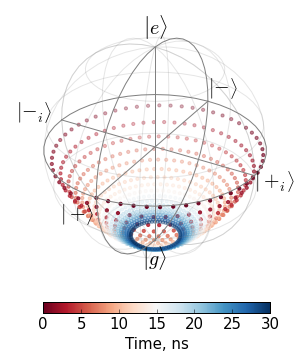
\includegraphics[width=0.95\textwidth]{Pictures/bloch_rel}
\caption{Релаксация,\\ $\gamma = 0.1,\ \gamma_\phi = 0$}
\end{subfigure}
\begin{subfigure}[t]{0.32\textwidth}
\centering
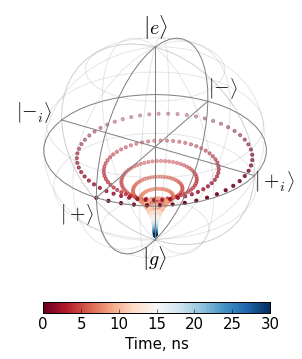
\includegraphics[width=0.95\textwidth]{Pictures/bloch_tot}
\caption{Общий эффект, \\$\gamma = \gamma_\phi = 0.1$}
\end{subfigure}
\begin{subfigure}[t]{0.32\textwidth}
\centering
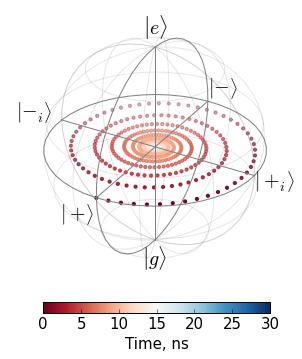
\includegraphics[width=0.95\textwidth]{Pictures/bloch_deph}
\caption{Дефазировка, \\ $\gamma = 0,\ \gamma_\phi = 0.1$}
\end{subfigure}
\caption{Диссипативная динамика кубита с $\nu_q$=1 ГГц.}
\label{fig:bloch}
\end{figure}

Для состояния $\ket{+} = \frac{1}{\sqrt{2}}(\ket{e}+\ket{g})$ более интересная картина эволюции представлена на \autoref{fig:bloch}. Как видно, дефазировка уничтожает когерентность системы, т.е. приближает значение $\Tr{\hat \rho_q^2}$ к нулю, гораздо быстрее, чем релаксация.
\chapter{Экспериментальная часть}
\chapter{Результаты}
\chapter{Заключение}

\bibliographystyle{ugost2008}
\bibliography{Thesis.bib}

\end{document}